\documentclass[12pt,a4paper]{article}

% Packages
\usepackage{amsmath}
\usepackage{subcaption}
\usepackage{amsfonts}
\usepackage{amssymb}
\usepackage{graphicx}
\usepackage[margin=1in]{geometry}
\usepackage{enumitem}
\usepackage[hidelinks]{hyperref}
\usepackage{xcolor}

% Title
\title{Homework Report for Computer Vision}
\author{Yu Xiang, Luo}
\date{\today}

\begin{document}

\maketitle

\[
	\href{https://github.com/YuXiangLo/Computer-Vision}{\text{\textcolor{blue}{You can check this github for more information}}}
\]

\begin{enumerate}[label=(\alph*)]
	\item Dilation\\
		\\
		\fbox{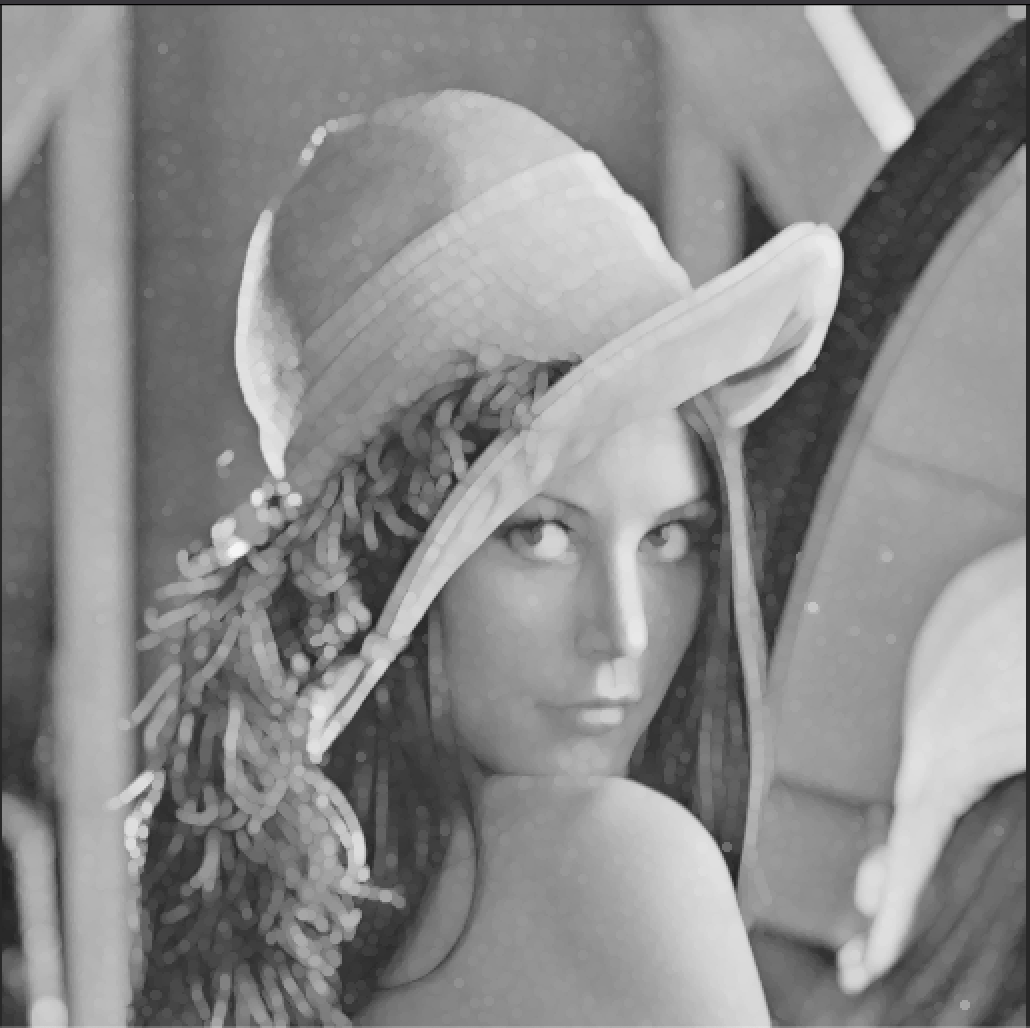
\includegraphics[width=0.4\textwidth]{img/dilation.png}}\\
		\\
		{\small Find the maximum value of pixel in kernel space and place it to the return image,
		since the large the value is, the lighter the pixel is.\\}
		\\
		\texttt{for pixel in kernel space:\\
		\text{\ \ \ \ }return\_pixel = max(return\_pixel, pixel)\\
		putpixel((x, y), return\_pixel) \textcolor{lightgray}{// put pixel to the center of the kernel}}
		\newpage
	\item erotion\\
		\\
		\fbox{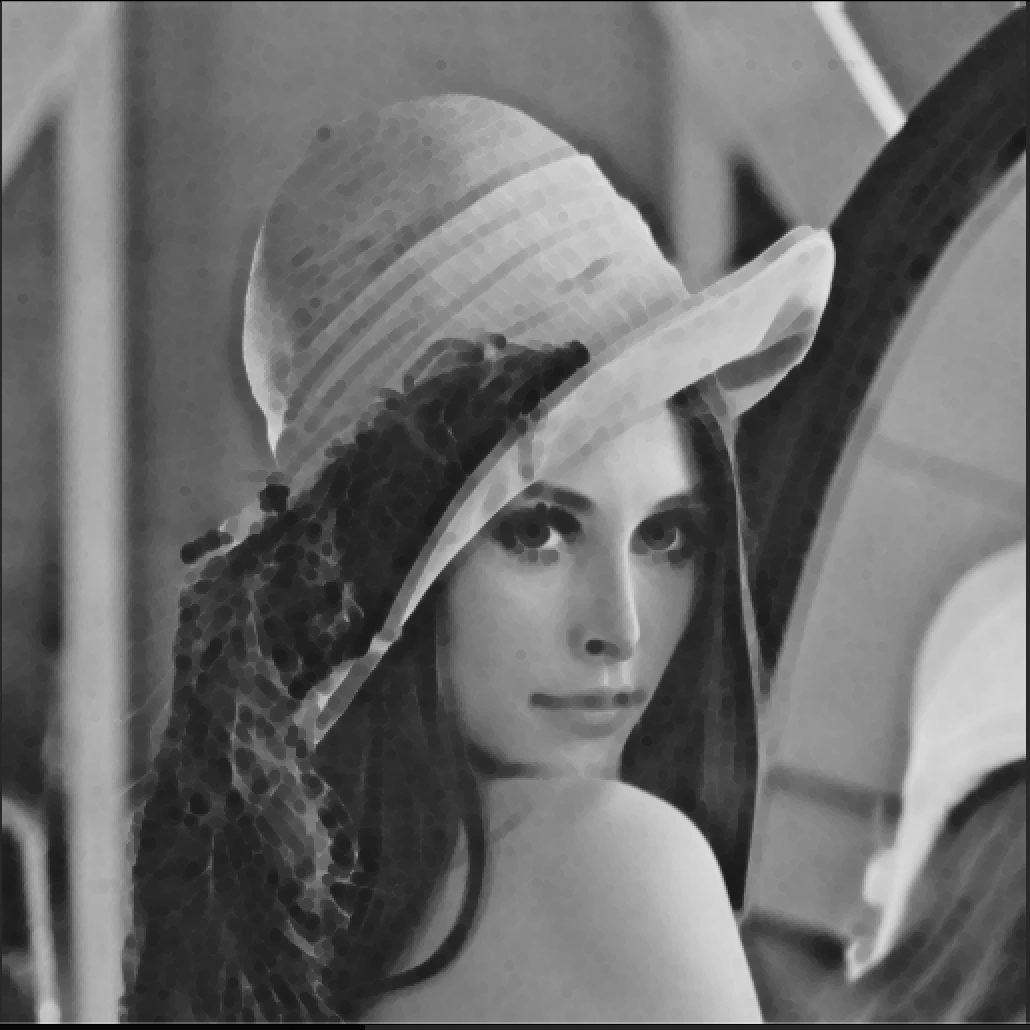
\includegraphics[width=0.4\textwidth]{img/erosion.png}}\\
		\\
		{\small Find the minimum value of pixel in kernel space and place it to the return image,
		since the smaller the value is, the darker the pixel is.\\}
		\\
		\texttt{for pixel in kernel space:\\
		\text{\ \ \ \ }return\_pixel = min(return\_pixel, pixel)\\
		putpixel((x, y), return\_pixel) \textcolor{lightgray}{// put pixel to the center of the kernel}}
	\item opening \& closing\\
		\\
		Combination of dilation and erosion.
		\begin{figure}[ht]
			\centering
            \begin{subfigure}{0.45\textwidth}
				\centering
				\fbox{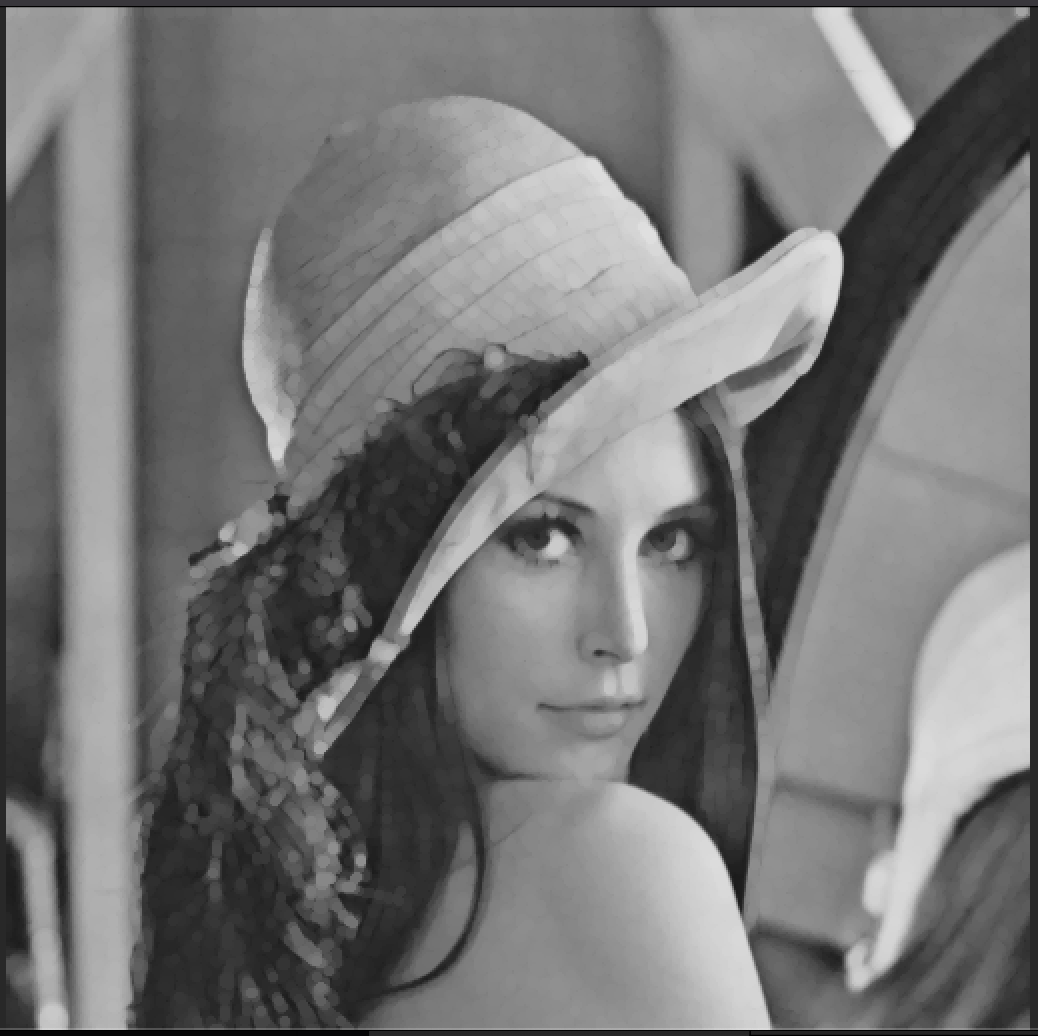
\includegraphics[width=\textwidth]{img/opening.png}}
				\caption{opening}
				\label{fig:subfig1}
			\end{subfigure}
			\hfill
			\begin{subfigure}{0.45\textwidth}
				\centering
				\fbox{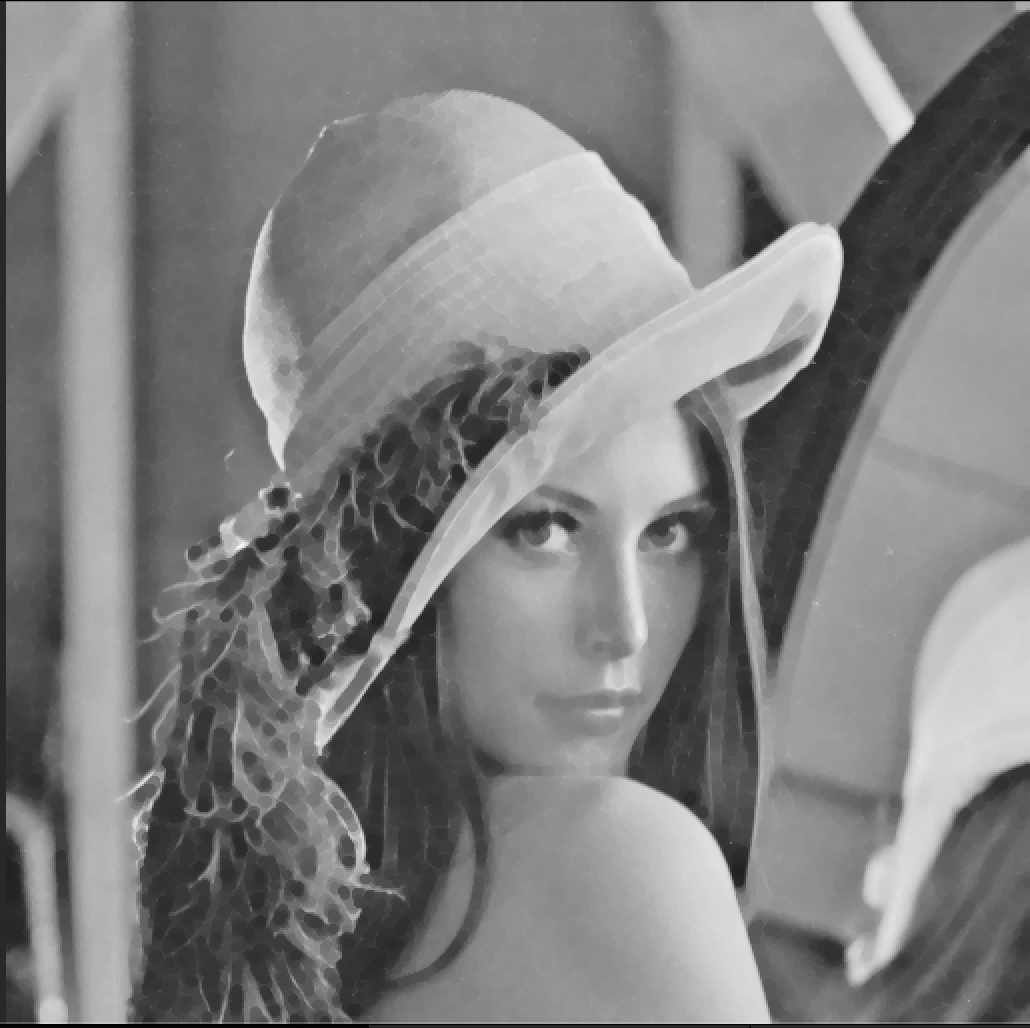
\includegraphics[width=\textwidth]{img/closing.png}}\\
				\caption{closing}
				\label{fig:subfig2}
			\end{subfigure}
		\end{figure}
		\newline
		\texttt{opening(image) = dilation(erosion(image))\\ closing(image) = erosion(dilation(image))}


		

\end{enumerate}



\end{document}
